\documentclass{beamer}
\usepackage{listings}
\usepackage{hyperref}
\usepackage{tikz}
\usetikzlibrary{positioning,shadows,arrows,shapes,calc}
\def\labelenumi\theenumi
\usepackage{graphicx}
\usepackage{amsmath}
\mode<presentation>{\usetheme{Frankfurt}}
\AtBeginSection
{
  \begin{frame}<beamer>
    \frametitle{Outline}
    \tableofcontents[currentsection,currentsubsection]
  \end{frame}
}
\title{Lecture 21: Barycentric Coordinates}
\author{Mark Hasegawa-Johnson\\All content~\href{https://creativecommons.org/licenses/by-sa/4.0/}{CC-SA 4.0} unless otherwise specified.}
\date{ECE 417: Multimedia Signal Processing, Fall 2020}  
\institute{University of Illinois}
\titlegraphic{\includegraphics{../../../17fall/lectures/imark_1867_bold.png}}
\begin{document}

% Title
\begin{frame}
  \maketitle
\end{frame}

% Title
\begin{frame}
  \tableofcontents
\end{frame}

%%%%%%%%%%%%%%%%%%%%%%%%%%%%%%%%%%%%%%%%%%%%%%%%%%%%%%%%%
\section{How to Make a Talking Head}
\setcounter{subsection}{1}

\begin{frame}
  \centerline{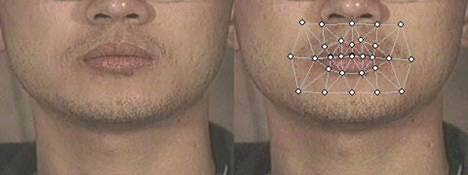
\includegraphics[height=1in]{mp7_image_warping_points.jpg}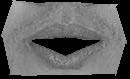
\includegraphics[height=1in]{mp7_image_warped.jpg}}
  {\bf Goal of MP4:} Generate video frames (right) by warping a static image (left).
\end{frame}

\begin{frame}
  \frametitle{Talking head, full outline}
  \centerline{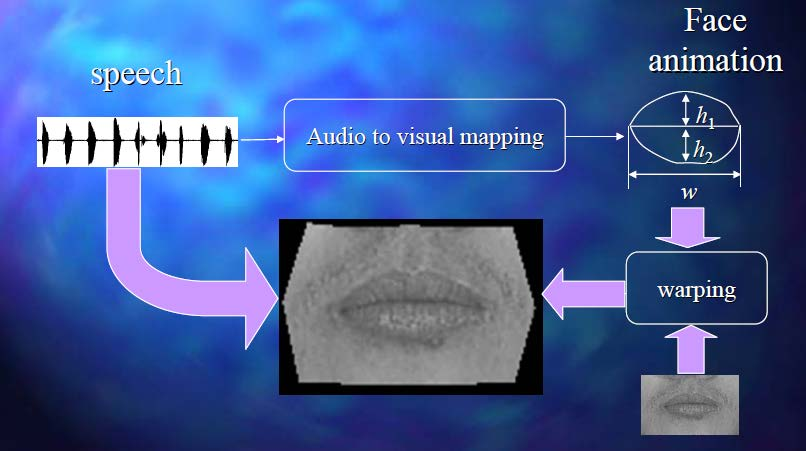
\includegraphics[width=4.5in]{mp7_image_warping.jpg}}
\end{frame}

\begin{frame}
  \frametitle{How it is done}
    \begin{align*}
      \mbox{lip\_height,width} &= \mbox{NeuralNet}\left(\mbox{MFCC}\right)\\
      \mbox{out\_triangs} &= \mbox{LinearlyInterpolate}\left(\mbox{inp\_triangs,lip\_height,width}\right)\\
      \mbox{inp\_coord} &= \mbox{BaryCentric}\left(\mbox{out\_coord,inp\_triangs,out\_triangs}\right)\\
      \mbox{out\_image} &= \mbox{BilinearInterpolate}\left(\mbox{inp\_coord,inp\_image}\right)
    \end{align*}
\end{frame}

%%%%%%%%%%%%%%%%%%%%%%%%%%%%%%%%%%%%%%%%%%%%%%%%%%%%%%%%%
\section{Barycentric Coordinates}
\setcounter{subsection}{1}

\begin{frame}
  \centerline{\href{https://www.youtube.com/watch?v=il6Z5LCykZk}{\includegraphics[width=4.5in]{../../../17fall/lectures/youtube_affine.png}}}
\end{frame}

\begin{frame}
  \frametitle{Piece-wise affine transform}
  \begin{itemize}
    \item OK, so somebody's given us a lot of points, arranged like
      this in little triangles.
    \item We know that we want a DIFFERENT AFFINE TRANSFORM for EACH
      TRIANGLE.  For the $k^{\textrm{th}}$ triangle, we want to have
      \[
      A_k = \left[\begin{array}{ccc}a_k&b_k&c_k\\d_k&e_k&f_k\\0&0&1\end{array}\right]
      \]
  \end{itemize}
  \centerline{\includegraphics[height=1in]{../../../17fall/lectures/mp7_image006.jpg}}
\end{frame}

\begin{frame}
  \frametitle{Piece-wise affine transform}
  \[
  \mbox{output point:}~\vec{x}=\left[\begin{array}{c}x\\y\\1\end{array}\right],~~~
  \mbox{input point:}~\vec{u}=\left[\begin{array}{c}u\\v\\1\end{array}\right]
  \]
  {\bf Definition}: if $\vec{x}$ is in the $k^{\textrm{th}}$ triangle in the
  {\bf output image}, then we want to use the $k^{\textrm{th}}$ affine transform:
  \[
  \vec{x}=A_k \vec{u},~~~\vec{u}=A_k^{-1}\vec{x}
  \]
  \centerline{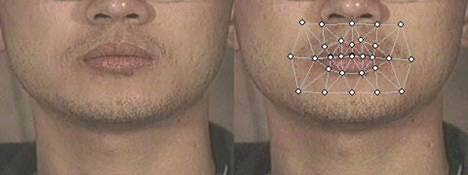
\includegraphics[height=1in]{mp7_image_warping_points.jpg}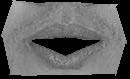
\includegraphics[height=1in]{mp7_image_warped.jpg}}
\end{frame}

\begin{frame}
  If {\bf it is known that} $\vec{u}=A_k^{-1}\vec{x}$ for some unknown
  affine transform matrix $A_k$,
  \vspace*{2mm}\\
  then
  \vspace*{2mm}\\
  the method of barycentric
  coordinates finds $\vec{u}$
  \vspace*{2mm}\\
  {\bf without ever finding} $A_k$.
\end{frame}

\begin{frame}
  \begin{columns}[t]
    \column{2.5in}
    \begin{block}{Barycentric Coordinates}
    Barycentric coordinates turns the problem on its head.  Suppose
    $\vec{x}$ is in a triangle with corners at $\vec{x}_1$,
    $\vec{x}_2$, and $\vec{x}_3$. That means that
    \[
    \vec{x}=\lambda_1\vec{x}_1+\lambda_2\vec{x}_2+\lambda_3\vec{x}_3
    \]
    where
    \[
    0\le\lambda_1,\lambda_2,\lambda_3\le 1
    \]
    and
    \[
    \lambda_1+\lambda_2+\lambda_3=1
    \]
    \end{block}
    \column{2.25in}
    \begin{block}{}
      \centerline{\includegraphics[width=2.25in]{../../../17fall/lectures/480px-TriangleBarycentricCoordinates.png}}
    \end{block}
  \end{columns}
\end{frame}

\begin{frame}
  \frametitle{Barycentric Coordinates}
  Suppose that all three of the corners are 
  transformed by some affine transform $A$, thus
  \[
  \vec{u}_1=A\vec{x}_1,~~
  \vec{u}_2=A\vec{x}_2,~~
  \vec{u}_3=A\vec{x}_3
  \]
  Then if
  \[
  \mbox{If:}~\vec{x}=\lambda_1\vec{x}_1+\lambda_2\vec{x}_2+\lambda_3\vec{x}_3
  \]
  Then:
  \begin{eqnarray*}
    \vec{u} &=& A\vec{x}\\
    &=& \lambda_1A\vec{x}_1+\lambda_2A\vec{x}_2+\lambda_3A\vec{x}_3\\
    &=& \lambda_1\vec{u}_1+\lambda_2\vec{u}_2+\lambda_3\vec{u}_3
  \end{eqnarray*}
  In other words, once we know the $\lambda$'s, we no longer need to
  find $A$.  We only need to know where the corners of the triangle
  have moved.
\end{frame}

\begin{frame}
  \begin{columns}[t]
    \column{2.5in}
    \begin{block}{Barycentric Coordinates}
      If
      \[
      \vec{x}=\lambda_1\vec{x}_1+\lambda_2\vec{x}_2+\lambda_3\vec{x}_3
      \]
      Then
      \[
      \vec{u}= \lambda_1\vec{u}_1+\lambda_2\vec{u}_2+\lambda_3\vec{u}_3
      \]
    \end{block}
    \column{2.25in}
    \begin{block}{}
      \centerline{\includegraphics[width=2.25in]{../../../17fall/lectures/480px-TriangleBarycentricCoordinates.png}}
    \end{block}
  \end{columns}
\end{frame}

\begin{frame}
  \frametitle{How to find Barycentric Coordinates}
  But how do you find $\lambda_1$, $\lambda_2$, and $\lambda_3$?
  \[
  \vec{x}=\lambda_1\vec{x}_1+\lambda_2\vec{x}_2+\lambda_3\vec{x}_3
  =\left[\vec{x}_1,\vec{x}_2,\vec{x}_3\right]
  \left[\begin{array}{c}\lambda_1\\\lambda_2\\\lambda_3\end{array}\right]
  =\left[\begin{array}{ccc}x_1&x_2&x_3\\y_1&y_2&y_3\\1&1&1\end{array}\right]
  \left[\begin{array}{c}\lambda_1\\\lambda_2\\\lambda_3\end{array}\right]
  \]
  Write this as:
  \[
  \vec{x}=X\vec\lambda
  \]
  Therefore
  \[
  \vec\lambda = X^{-1}\vec{x}
  \]
  This {\bf always works:} the matrix $X$ is always invertible, unless
  all three of the points $\vec{x}_1$, $\vec{x}_2$, and $\vec{x}_3$
  are on a straight line.
\end{frame}
\begin{frame}
  \frametitle{How do you find out which triangle
    the point is in?}
  \begin{itemize}
  \item Suppose we have $K$ different triangles, each of which is
    characterized by a $3\times 3$ matrix of its corners
    \[
    X_k = \left[\vec{x}_{1,k},\vec{x}_{2,k},\vec{x}_{3,k}\right]
    \]
    where $\vec{x}_{m,k}$ is the $m^{\textrm{th}}$ corner of the
    $k^{\textrm{th}}$ triangle.
  \item Notice that, for any point $\vec{x}$, for ANY triangle $X_k$,
    we can find
    \[\lambda = X_k^{-1}\vec{x}\]
  \item However, the coefficients $\lambda_1$, $\lambda_2$, and
    $\lambda_3$ will all be between $0$ and $1$ {\bf if and only if}
    the point $\vec{x}$ is inside the triangle $X_k$.  Otherwise, some
    of the $\lambda$'s must be negative.
  \end{itemize}
\end{frame}

\begin{frame}
  \frametitle{The Method of Barycentric Coordinates}
  To construct the animated output image frame $J[y,x]$, we do
  the following things:
  \begin{itemize}
  \item First, for each of the reference triangles $U_k$ in the input
    image $I(u,v)$, decide where that triangle
    should move to.  Call the new triangle location $X_k$.
  \item Second, for each output pixel $(x,y)$:
    \begin{itemize}
    \item For each of the triangles, find $\vec\lambda=X_k^{-1}\vec{x}$.
    \item Choose the triangle for which all of the $\lambda$ coefficients
      are $0\le\lambda\le 1$.
    \item Find $\vec{u}=U_k\vec\lambda$.
    \item Estimate $I(u,v)$ using bilinear interpolation.
    \item Set $J[y,x]=I(v,u)$.
    \end{itemize}
  \end{itemize}
\end{frame}

\section{Conclusion}
\setcounter{subsection}{1}

\begin{frame}
  \centerline{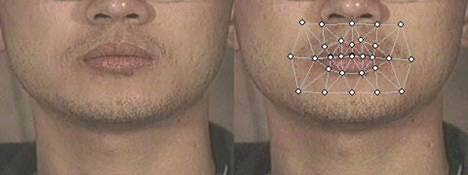
\includegraphics[height=1in]{mp7_image_warping_points.jpg}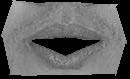
\includegraphics[height=1in]{mp7_image_warped.jpg}}
  \begin{align*}
    \mbox{lip\_height,width} &= \mbox{NeuralNet}\left(\mbox{MFCC}\right)\\
    \mbox{out\_triangs} &= \mbox{LinearlyInterpolate}\left(\mbox{inp\_triangs,lip\_height,width}\right)\\
    \mbox{inp\_coord} &= \mbox{BaryCentric}\left(\mbox{out\_coord,inp\_triangs,out\_triangs}\right)\\
    \mbox{out\_image} &= \mbox{BilinearInterpolate}\left(\mbox{inp\_coord,inp\_image}\right)
  \end{align*}
\end{frame}

\begin{frame}
  \frametitle{Barycentric Coordinates}

  \begin{itemize}
  \item For each of the triangles, find $\vec\lambda=X_k^{-1}\vec{x}$.
  \item Choose the triangle for which all of the $\lambda$ coefficients
    are $0\le\lambda\le 1$.
  \item Find $\vec{u}=U_k\vec\lambda$.
  \item Estimate $I(v,u)$ using bilinear interpolation.
    \[
    I(v,u) = \sum_m\sum_n I[n,m] h(v-n,u-m)
    \]    
  \item Set $J[y,x]=I(v,u)$.
  \end{itemize}
\end{frame}


\end{document}

